\section{System architecture overvirw}

\begin{figure}[!ht]
    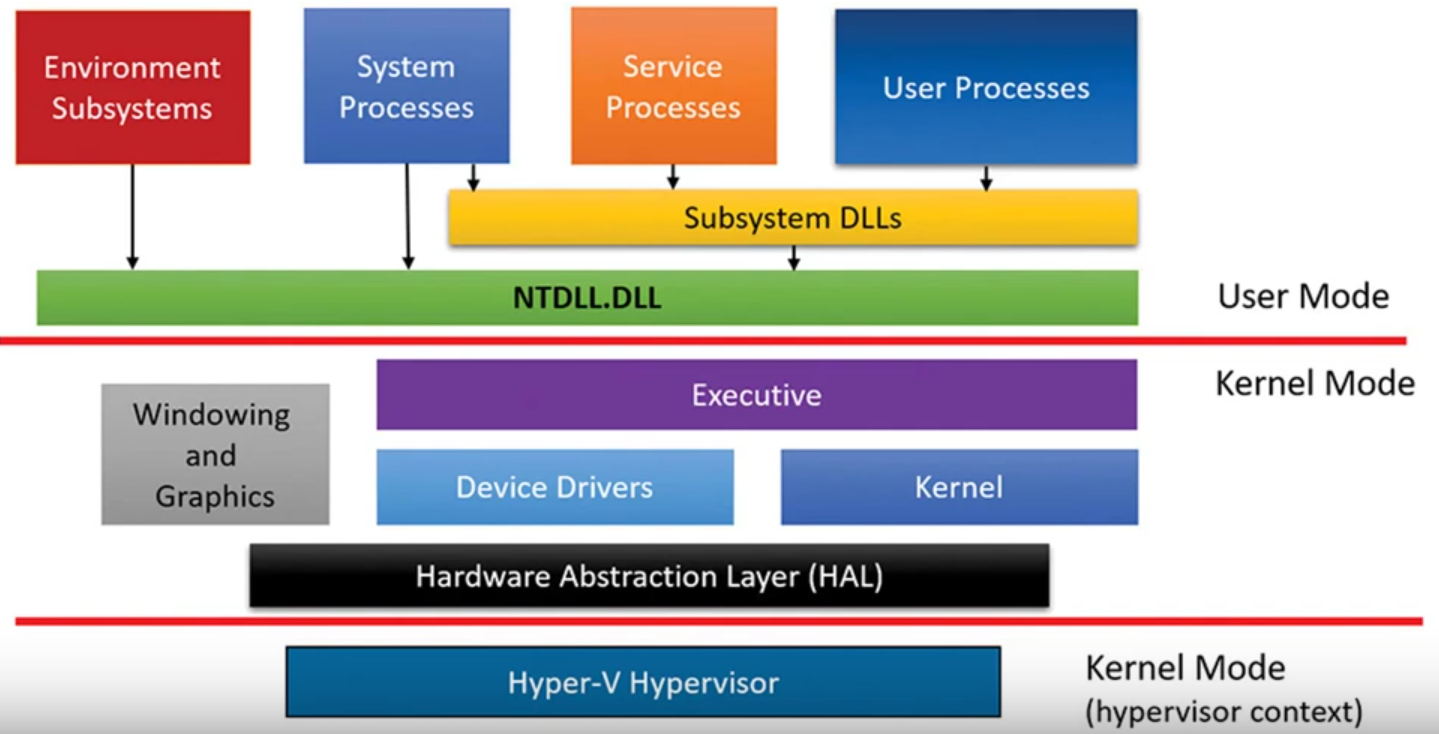
\includegraphics[width=\linewidth]{knowledge/internals/images/simplified-archi.png}
    \caption{Simplified archi}
    \label{fig:windows_siplified_archi}
\end{figure}

\begin{itemize}
    \item user-mode:
        \begin{itemize}
            \item {\bf Service processes} are processes that host Windows services, such as the Task Scheduler and Print Spooler services
            \item {\bf System processes} are fixed, or hardwired, processes, such as the logon process and the Session Manager, that are not Windows services. That is, they are not started by the {\bf Service Control Manager}
            \item Environment subsystem server processes implement part of the support for the OS environment, or personality, presented to the user and programmer. 
        \end{itemize}
    \item kernel-mode:
        \begin{itemize}
            \item {\bf Executive (\verb+Ntoskrnl.exe+)} contains the base OS services, such as memory management, process and thread management, security, I/O, networking, and inter-process communication.
            \item {\bf Windows kernel (\verb+Ntoskrnl.exe+)} consists of low-level OS functions, such as thread scheduling, interrupt and exception dispatching, and multiprocessor synchronization. It also provides a set of routines and basic objects that the rest of the executive uses to implement higher-level constructs.
            \item {\bf Device drivers} includes both hardware device drivers, which translate user I/O function calls into specific hardware device I/O requests, and non-hardware device drivers, such as file system and network drivers.
            \item {\bf Hardware Abstraction Layer (HAL)(\verb+hal.dll+)}  layer of code that isolates the kernel, the  device drivers, and the rest of the Windows executive from platform-specific hardware differences (such as differences between motherboards).
            \item {\bf windowing and graphics system (\verb+Win32k.sys+)} implements the graphical user interface (GUI) functions (aka Windows USER and GDI functions), such as dealing with windows, user interface controls, and drawing.
            \item {\bf hypervisor layer (\verb+hdvix64.exe+, \verb+hvax64.exe+)} is composed of a single component: the hypervisor itself. he hypervisor is itself composed of multiple internal layers and services, such as its own memory manager, virtual processor scheduler, interrupt and timer management, synchronization routines, \ldots.
        \end{itemize}
\end{itemize}


\verb+ntdll.dll+ : Internal support functions and system service dispatch stubs to executive functions

\verb+kernel32.dll, advapi32.dll, user32.dll,gdi32.dll+: core windows subsystem dlls